%\section{ Hamiltonian theory}
%\label{sec:theory}
The wave-particle interaction is described on the local cells 
at position $s$ along the dipole field, with phase space characterized by new canonical coordinates $(\xi$, $\Omega)$
\cite{zheng2024}.
The Hamiltonian of resonant electrons in the frame of reference moving with the local resonance for the onset of chorus is 
%is obtained through canonical transformation 
\cite{zheng2024}
%.  In the original Hamiltonian, $\xi$, $\Omega$ phase space is decoupled for each cell at position $s_i$ along the magnetic field. In our hybrid Vlasov simulation \cite{zheng2023b,zheng2024}, we separately examine the phase flow for the onset of chorus using the following Hamiltonian,
\begin{equation}\label{eq.H_lab}
    K = \frac{k_l^2\Omega^2}{2} + {\Re}\left(\frac{\omega_b^2}{k_l^2} e^{-\imath \xi} + \frac{\omega_b^2}{k_l^2}\alpha \cdot \xi \right)~,
\end{equation}
where ${\Re}$ denotes taking the real part.
%We analyze 
The inhomogeneous parameter $\alpha$ satisfies
\begin{equation}\label{eq.alpold}
   \alpha  = \frac{k_l}{\omega_b^2}(\mathcal{J} - \frac{\Pi}{2}) \frac{d\omega_{ce}}{ds}~,
\end{equation}
and the bounce frequency satisfies
\begin{equation}
    \frac{\omega_b^2}{k_l^2} =  a(s,t) \sqrt{2\omega_{ce}\mu(s)}~,
\end{equation}
where $\mu(s) = \mathcal{J}(s)+\Pi(s)+\Omega$
relates to 
the magnetic moment.
%$\mu = \mathcal{J}+\Pi+\Omega$. 
Note that $\mathcal{J}$ is another canonical momentum associated with the slow-scale motion along the field line. The cyclotron frequency $\omega_{ce}$
and parameter $\Pi = (\omega - \omega_{ce})/k_l^2$ from the canonical transformation  are determined from the background plasma parameters on each local cell \cite{zheng2024,zheng2023b}, 
% The background magnetic field and $\Pi$ parameters are
as shown in Figs. \ref{fig.aanda}(a) and \ref{fig.aanda}(b).
%\begin{figure}
%    \centering
%    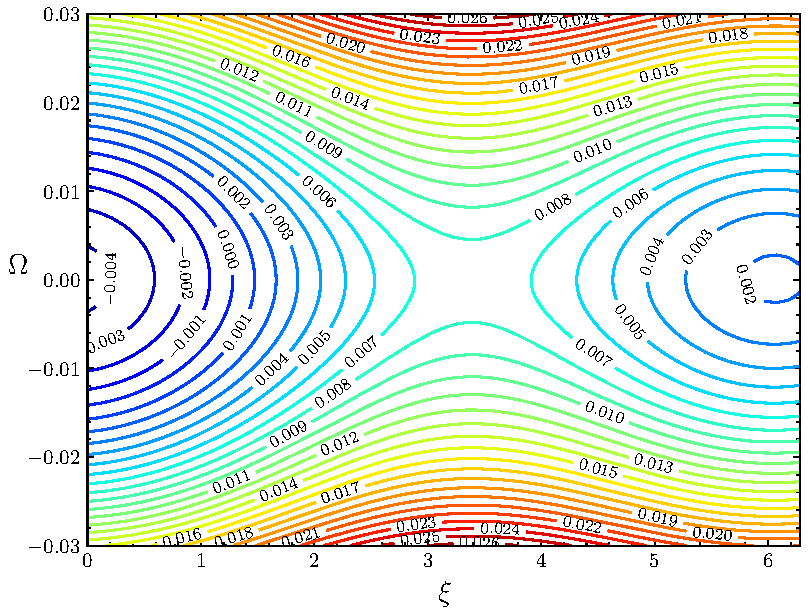
\includegraphics[scale=0.5]{img/Hamcontour.pdf}
%    \caption{The contour plot of Hamiltonian in Eq. (\ref{eq.H_lab}) (a) and  Eq. (\ref{eq.H_frame}) (b) using fixed $\mathcal{J}, a, \Pi$ parameters. The dots and red cross denotes the initial location for the test particle tracing.
%    \label{fig.Hamcontour}
%    }
%\end{figure}
%add background, 
%wave instability: tempterature anisotropy, 
%with inhomogeneous field : field line from upstream to downstream
%electrons move from downstream to upstream, wave move in opposite direction, k along B field line
%In the magnetosphere, the chorus is triggered by the unstable whistler wave \cite{omura_theory_2008,tao_theoretical_2020}. 
%The most unstable whistler wave with frequency $\omega_l$ and wave number $k_l$ is the seed wave for triggering the chirping chorus.
To study the onset of the chorus, we choose the reference frame fixed at the frequency  $\omega_l$ and wave number $k_l$  of the most unstable whistler wave which is excited from the electron temperature anisotropy \cite{gary_1993}. 
Since $\omega_l$ and $k_l$ are constant in time, we refer such reference frame as the static resonance frame. 
The  wave envelope of the vector potential $a$ becomes a complex number with an additional phase $\delta \phi$ since the static frame can not exactly follow the real-time resonance. 
The complex wave vector potential $a$ is written as 
\begin{equation}
    a(s,t) = |a(s,t)| \cdot e^{\imath \delta \phi(s,t)}~.
\end{equation}
Therefore, we take the real part in the wave-particle interaction term in the  Hamiltonian Eq. (\ref{eq.H_lab}).
%Here we show the wave data from 
In the Vlasov simulation,
 the wave propagates along the background magnetic field from upstream to the downstream region.
The resonant electrons 
move opposite to the motion of the wave packet.  
%are moving in opposite direction along the field line.
% in Fig. \ref{fig.aanda}.
The frequency chirping can be seen from Fig. \ref{fig.aanda}(c) where the additional phase $\delta \phi$ results in a modulation on the wave envelope.
The chorus wave is triggered in the source region near the equator and propagates to the downstream where  a prominent wave envelope forms in the propagation region, as shown in Fig. \ref{fig.aanda}(d).


%\begin{equation}\label{eq.cell_j}
%    (\omega_l - \omega_{ce})\mathcal{J} +  \frac{(\omega_l - \omega_{ce})^2}{2k_l^2} = \mathrm{Const.}
%\end{equation}
%Since we consider the parallel propagating wave, 
%%the cell is aligned with the field line, and 
%the reference frame moves according to the 
%resonance 
%velocity,
%\begin{equation}\label{eq.cell_s}
%    \frac{d s_i}{d t} = \frac{\omega_l-\omega_{ce}}{k_l}~.
%\end{equation}

\begin{figure}
    \centering
    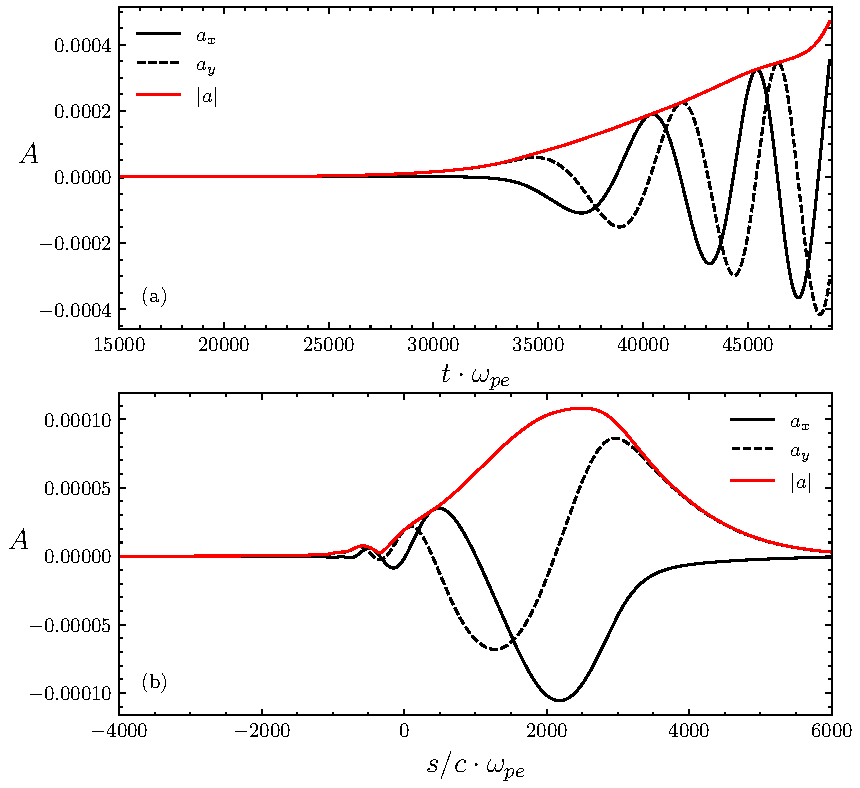
\includegraphics[scale=0.5]{img/aanda.pdf}
    \caption{Variation of (a) $\omega_{ce}$ and (b) $\Pi$ along the dipole field line.  (c) Time evolution and (d) spatial distribution of the orthogonal components of vector potential, $a_x$ and $a_y$, and the amplitude $|a|$ in the simulation.
    \label{fig.aanda}
    }
\end{figure}

%In other word, $a$ is a complex number and so does $\omega_b$.
The phase space trajectory can be obtained from the Hamilton's  equation,
\begin{equation}\label{eq.lab_eq}
    \begin{aligned}
        \frac{d\Omega}{dt} &= - \sqrt{2\omega_{ce}(s)\mu(s)} {\Im} (a(s,t)\cdot e^{-\imath \xi}) - \frac{\omega^2_{b}}{k_l^2(s)} \alpha
        \\
        \frac{d\xi}{dt} &= k_l^2(s) \Omega +\sqrt{\frac{\omega_{ce}(s)}{2\mu(s)}} {\Re}(a(s,t)\cdot e^{-\imath \xi})
    \end{aligned}
\end{equation}
where $\Im$ denotes taking the imaginary part.
%particle trajectory
With the calculated wave fields  in the Vlasov simulation \cite{zheng2024}, we solve the  equations of motion Eq. (\ref{eq.lab_eq})
%and show the time variation of the particle's phase space coordinates in Fig. \ref{fig.phaseflow}.
%We choose a test particle, initially locate at $s_0 \simeq 2106.9 c/\omega_{pe}$ and $t_0 \simeq 36675 \omega_{pe}^{-1}$, and we set the particle to been initially trapped at the resonance center $\xi = 6, \Omega \simeq 5.4\times10^{-4}$. 
%Starting from the initial location $s_0$, we push the phase flow to $t_0 + \Delta T$, where $\Delta T= 48.9 \omega_{pe}^{-1}$,
 using time-adaptive Runge-Kutta method. Then we push the resonant particle along the field line according to their characteristic lines in $s$-$\mathcal{J}$ space.
%The procedure is in accordance with our Euler-Lagrangian hybrid Vlasov method.
In the static resonance frame, the trapped particle does not have a closed phase space trajectory and their angle variable $\xi$ is shifting and matching with the wave phase $\delta \phi$ along its trajectory, as illustrated in Fig. \ref{fig.phaseflow}(a). This is in accordance with the phase locking condition \cite{tao_trap-release-amplify_2021}.
The varying phase $\delta \phi(s,t)$ also indicates the acceleration of trapped particles along $\Omega$ momentum dimension in phase space.
The momentum of the particle, as shown in Fig. \ref{fig.phaseflow}(b), is accelerating upwards along $\Omega$ dimension due to the rising tone frequency chirping.

\begin{figure}
    \centering
    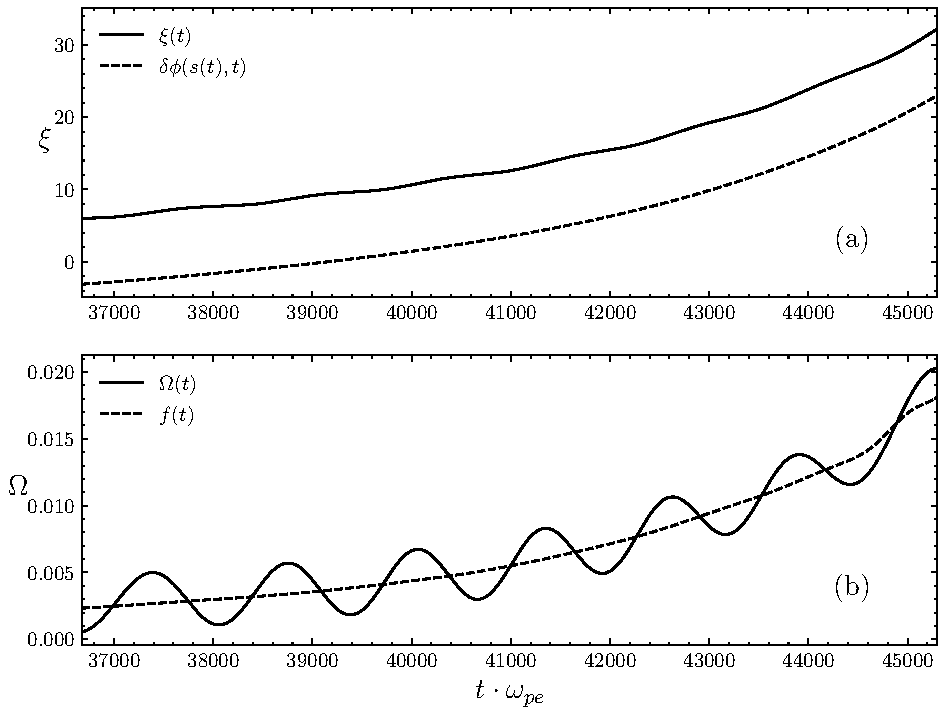
\includegraphics[scale=0.5]{img/phaseflow.pdf}
    \caption{
    %(a) Phase space trajectories of  test particles with initial angle $\xi = 6$ sampled in $\Omega \in [-0.01,0.01]$, 
    (a) Typical variation of angle coordinate $\xi$ of a test particle and the  wave phase $\delta \phi$ along its trajectory.  (b) Particle momentum $\Omega$ versus time. The dashed line denotes Eq. (\ref{eq.ft}).
    \label{fig.phaseflow}
    }
\end{figure}
\begin{figure}
    \centering
    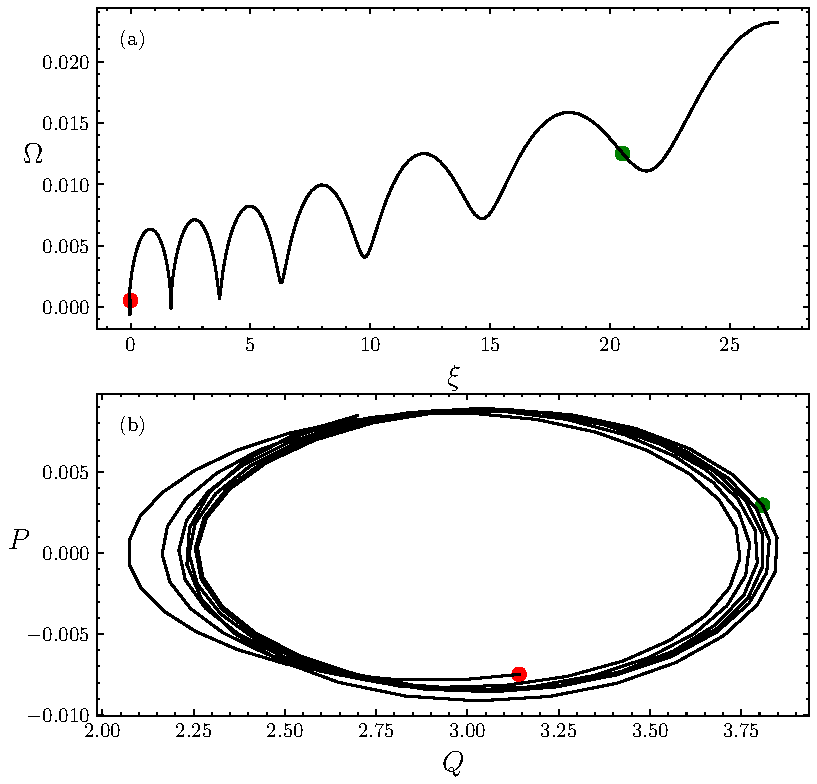
\includegraphics[scale=0.5]{img/Trajectory.pdf}
    \caption{Phase space trajectory of a test particle from $s \simeq 2107 c/\omega_{pe}$ at $t\simeq 36675 \omega_{pe}^{-1}$ 
    (red dots)
     to $s \simeq 205 c/\omega_{pe}$ at $t=45476 \omega_{pe}^{-1}$ 
    (green dots)
      in the (a) static  and  (b) real-time frames.  The corresponding enclosed phase space loop of a particle in the (c)  static and  (d) real-time  frames. 
      %at different times. The red and green dots and  denote 
      %during the time period during which the particles are trapped. 
%    The start point, and the green dot denotes $t \simeq 44498  \omega_{pe}^{-1}$ which is the critical point where the adiabatic invariant changes significantly.
    \label{fig.traj} 
    }
\end{figure}

Since the wave phase $\delta \phi$ can be calculated from the Vlasov simulation
 \cite{zheng2024}, we can construct a canonical transformation to shift the static resonance frame to the real-time resonance frame.
The new canonical variables take the form \cite{berk1999},
\begin{equation}
    \begin{aligned}
        Q &= \xi - \delta \phi(s(t),t)~,
        \\
        P & = \Omega - f(t)~,
    \end{aligned}
\end{equation}
where $f(t)$ is a time dependent function to be determined.
The canonical  transformation corresponds to a type-2 generating function
\begin{equation}
    F_2(\xi,P,t) = (\xi - \delta \phi) \cdot P + \xi \cdot f(t)
\end{equation}
and the corresponding new Hamiltonian  is
\begin{equation}
    \begin{aligned}
        &  K^\prime = K + \frac{\partial F_2}{\partial t}
        \\
        & = \frac{k_l^2}{2}(P+f(t))^2 
        + \sqrt{2\omega_{ce}(\mathcal{J}+P+f(t)+\Pi)} \cdot |a|\cos Q 
        \\
        & + \left(\frac{1}{k_l}\left(\mathcal{J} - \frac{\Pi}{2} \frac{d\omega_{ce}}{ds}\right)  +\frac{d f(t)}{d t} \right)\cdot(Q + \delta \phi)  - \frac{d \delta \phi}{d t} P ~. 
        \end{aligned}
\end{equation}
In addition,  the first order term with respect to $P$  should be eliminated in the  Hamiltonian, which determines $f(t)$ as
\begin{equation}\label{eq.ft}
    \begin{aligned}
    f(t) & = \frac{1}{k_l^2} \frac{d \delta \phi}{d t}  &= \frac{\delta \omega - v_r \delta k}{k_l^2}~.
    \end{aligned}
\end{equation} 
%Note that 
The total time derivative is evaluated along the particle trajectory, $d/dt = \partial/\partial t + v_r \partial /\partial s$ with $\delta \omega  \equiv \partial \delta \phi/\partial t$ and $\delta k  \equiv -\partial \delta \phi/\partial s$.
%We can examine Note that $f(t)$ is the first-order variation of $\Omega(\omega,k)$ due to the chirping frequency $\delta \omega$ and the wave number $\delta k$.
The expression Eq. (\ref{eq.ft}) agrees with the change of $\Omega$ in the test particle simulation shown in Fig. \ref{fig.phaseflow}(b).
%\begin{equation}
%    \begin{aligned}
%    \delta \omega & \equiv \frac{\partial \delta \phi}{\partial t}~,
%    \\
%    \delta k & \equiv -\frac{\partial \delta \phi}{\partial s}~,
%    \end{aligned}
%\end{equation}
For the derivative of $f(t)$, we only keep the term up to the first order, which gives
\begin{equation}
    \frac{d f(t)}{d t} \simeq \frac{1}{k_l^2}(\frac{\partial \delta \omega}{\partial t} + 2 v_r \frac{\partial \delta \omega}{\partial s} + \frac{3}{2}v_r\frac{\delta k}{k_l} \frac{d \omega_{ce}}{d s}  ).
\end{equation}
Finally, the new Hamiltonian takes the  form 
\begin{equation}\label{eq.H_frame}
    K^\prime = \frac{k_l^2 P^2}{2} + \frac{{\omega^\prime_{b}}^2}{k_l^2} \cos Q +\frac{{\omega^\prime_{b}}^2}{k_l^2} \alpha^\prime \cdot Q~,
\end{equation}
where 
%the new bounce frequency $\omega^\prime_{b}$ satisfies
\begin{equation}
    \frac{{\omega^\prime_{b}}^2}{k_l^2} = \sqrt{2\omega_{ce}(\mathcal{J}+P+f(t)+\Pi)}  |a|
\end{equation}
and 
%the new $\alpha^\prime$ satisfies
\begin{equation}\label{eq.alpnew}
    \begin{aligned}
    \frac{{\omega^\prime_{b}}^2}{k_l^2}\alpha^\prime & = \frac{1}{k_l}\left(\mathcal{J} - \frac{\Pi}{2}\right) \frac{d\omega_{ce}}{ds} \\
    & + \frac{1}{k_l^2}\left(\frac{\partial \delta \omega}{\partial t} + 2 v_r \frac{\partial \delta \omega}{\partial s} + \frac{3}{2}v_r\frac{\delta k}{k_l} \frac{d \omega_{ce}}{d s}\right)~.
    \end{aligned}
\end{equation}
The modified parameters describe the frequency chirping and 
the background magnetic field inhomogeneity.
%inhomogeneities in the background magnetic field, and 
The additional terms in Eq. (\ref{eq.alpnew}) compared to Eq.~(\ref{eq.alpold}) are the first order correction related to the frequency chirping and wave number variation.


%Using the wave data from our Vlasov simualtion, we show the contour plot both of the Hamiltonian (\ref{eq.H_lab}) and the modified Hamiltonian (\ref{eq.H_frame}) in Fig. \ref{fig.Hamcontour}. Due to the $\alpha$/$drg$ term in the Hamiltonian, the trapped region is enclosed between a saddle point  and a C point.
 Using the new Hamiltonian, we are able to consider  the particle dynamics in the real-time resonance frame
 where the Hamilton's equations have the same form as those in Eq.~(\ref{eq.lab_eq}) with the replacement
$\xi$ to $Q$,
$\Omega$ to $P$,
$\alpha$ to  $\alpha^\prime$, and 
${\omega_{b}}$ to ${\omega^\prime_{b}}$.
%only substitution of the parameter to new $\alpha^\prime$ and ${\omega^\prime_{b}}$.
%Now, for the new Hamiltonian, we solve the trajectory for a similar trapped test particle from the same temporospatial location $s_0,t_0$. 
%We compare the phase space trajectory with that in the static frame in Fig. \ref{fig.traj}.
%We show the corresponding Hamiltonian at this location in Fig. \ref{fig.Hamcontour}.
%It can be found that 
%Unlike in the static  resonance frame where the particle suffers a rapid change in $\Omega$ for each bounce in accordance with  Fig. \ref{fig.phaseflow}(b), there exists only a slight change when we track the particle in the real-time resonance frame, which demonstrates the effectiveness of the canonical transformation.
To show the differences, we choose a test particle initially at the resonance center and calculate its phase space trajectories in the different reference frames. In the static resonance frame, the particle suffers a rapid change in $\Omega$  for each bounce, as seen   in Fig. \ref{fig.traj}(a). In constrast, there exists only a slight change when we track the particle in the real-time resonance frame, as shown in Fig. \ref{fig.traj}(b), which demonstrates the effectiveness of the canonical transformation.

